\chapter{Contribution}\label{chap:contribution}
This thesis shall be understood as an extension to the works of Evermann et al. \cite{evermann2016} and Schönig et al. \cite{schoenig2018}, both of which were thoroughly presented in the previous section. The two works have demonstrated the applicability of LSTM neural networks in Predictive Process Monitoring, but have left out general perspectives on the sequence prediction problem.
We want to introduce said general perspective through adapting of the approach of Shibata et al. \cite{shibata2016bipartite} for Predictive Process Monitoring in \autoref{sec:contrib:nlp-inspiration}. During development, we realized that there are highly divergent understandings regarding the data input of neural networks for next-element predictions with sequences. Our contribution in this area is described in \autoref{sec:contrib:input-formatting}. We tie both topics together by providing a simple training framework in \autoref{sec:contrib:training-framework}. With it, we hope to facilitate a step towards result comparability. 

This chapter shall begin in \autoref{sec:contrib:case-sequence-understanding} with the theoretic underpinning that enables the work mentioned above: the understanding of a case trace as a sequence.\\

\section{Understanding a trace as a sequence}
\label{sec:contrib:case-sequence-understanding} 
The definition for sequences presented in \autoref{sec:background:sequence-prediction} needs to be extended so that a case trace can be understood as a sequence.

In the previous definition, the set $I$ had been used for \textit{items}, out of which itemsets are comprised. In this extension, an itemset represents a single row in a log. As such a row is made up of multiple different elements and adheres to a fixed schema, the definition needs to account for these two properties.\\

First, the set $I$ is now understood as a union of the sets $C_i$ which make up the distinct values inside one of the $n$ columns of a trace:
$$I = \bigcup\limits_{i=1}^{n} C_{i}$$

Second, each itemset $s$ needs to be bound by a specific schema. The schema needs to match the schema of the log and can be defined as such: $s = <i_1, i_2 ..., i_i>$ with $i_i \in C_i$. Thus, the original condition $s \subseteq I$ still holds true, but every item now has a fixed place in the itemset depending on which column it originates from.

\section{Taking inspiration from approaches in NLP}
\label{sec:contrib:nlp-inspiration}
Shibata et al.'s bipartite network architecture in combination with engineered SP-2 features has shown extraordinary performance in the SPiCE competition \cite{web:spice}. Under the hypothesis that a case can exhibit properties similar to grammatical rules, we test it in the business process domain. Furthermore, we consider sub-sequence information as proposed by Klinkmüller et al.~\cite{klinkmuller2018reliablemonitoring} as an alternative to the SP-2 features.

The two variations are henceforth referred to as SP2 for the bipartite architecture using SP-2 features and PFS for the bipartite architecture using sub-sequence information. They are compared to the performance of implementations that mimic Evermann et al. and Schönig et al. Where original performance statistics were published, these are used additionally. The BPIC2011 \cite{BPIC2011} and BPIC2017 \cite{BPIC2017} datasets are used and preprocessed differently as per each approach.\\

In \autoref{fig:sp2-pfs-architecture}, the SP2 and PFS architecture is displayed. While the general architecture has been adapted by Shibata et al., important details were taken from Schönig et al.

\begin{figure}
    \centering
    
\includegraphics[width=0.7\textwidth]{gfx/sp2-network-architecture.png}
    \caption{The SP2 and PFS networks share the architecture but inject different features.}
    \label{fig:sp2-pfs-architecture}
\end{figure}

Both SP2 and PFS models use $n$ units on the first input layer denoting the number of features for the encoded activities, timestamps and other event attributes. Both put out the next activity in one-hot encoded form through $m$ units, thus modelling the task as a multi-classification problem.

In contrast to Evermann et al. and Shibata et al., the number of units $m+n$ in the LSTM layers is a function of the input unit count and the output unit count. This follows general advice not to introduce bottlenecks in the hidden layers by using fewer units than required in the output layer. Furthermore, dropout layers have been introduced to prevent overfitting.

The SP2 and PFS features are fed in higher up on the right side of the tree, passing through a ReLU-activated, fully-connected layer, before the intermediate values are concatenated. Finally, the concatenated vectors are processed by fully-connected layers, with the commonly used Softmax activation function producing the final classification.

\section{Contrasts among sequence input formats}
\label{sec:contrib:input-formatting}
We implemented the SP2 and PFS variants as well as the comparison models using Python and the Keras neural networks API. While doing so, a wide range of recommended approaches to training the models were noted in relevant publications and on online platforms such as StackOverflow.\\

While some recommend sliding window approaches, others deem this against the concept of LSTM cells. Especially, Klinkmüller et al. argue against it: "[...]the popular strategy of cutting traces to certain prefix lengths to learn prediction models for ongoing instances is prone to yield unreliable models"~\cite{klinkmuller2018reliablemonitoring}. Again others argue that padding sequences to equal length makes training faster and does not affect accuracy. Furthermore, the batch size represents an important hyper-parameter, and no guidelines how to sort traces into batches were found. We believe that the understanding of the merits of each approach is of general value to any application of sequence prediction and make it part of our contribution.\\

When using Keras' implementation of LSTM, it is stateful \textit{during} a batch, and resets the internal state before the next one, unless specified otherwise. For the sake of simplicity, it is advisable to keep related data inside a single batch. Translated to traces, this means keeping a trace completely inside a batch. The Keras LSTM layers expect data to arrive in a three-dimensional array, where each dimension has a defined meaning:

$$(n_{samples}, n_{timesteps}, n_{features})$$

Each sample contains a number of timesteps $n_{timesteps}$ containing a number of features $n_{features}$, which is a constant. For each sample, the LSTM layer maintains a separate state, meaning that several traces can be trained on simultaneously~\cite{web:keras-lstm-state}. This definition opens up a range of possibilities, four of which we are investigating here.\\

First and easiest, one trace can be trained per batch.

Secondly, \textit{some} traces can be trained inside a single batch. This is possible if all traces inside one batch have the same number of timesteps, i.e. have the same length. The number of samples and timesteps may vary between batches. A look at a trace length distribution in \autoref{fig:bpic2011-length-distribution} reveals that grouped batching might bias the model toward longer traces who are smaller in number as they are trained batches of their own.

Third, there is the possibility of padding the number of time-steps in a sequence to the same length and use a Masking\footnote{\url{https://keras.io/layers/core/\#masking} (last visited on December 12, 2018)} layer to then filter out the padded values during training. This is likely to incur a performance hit due to the higher memory requirements for padded samples and processing overhead for filtering.

Fourth and finally, there is also the possibility to split the trace into samples by sliding a window along it. This results in $l-w+1$ samples for a trace of length $l$ and a window width $w$. Taking \autoref{tab:sliding-window} in \autoref{sec:background:feature-engineering} as an example, the window would be two timesteps wide. While this approach solves the problem of unequal sample lengths and facilitates batch construction, the model can only use a maximum of $w$ timesteps per sample for training, thus losing potential long-term dependencies. As both Evermann et al.~\cite{evermann2016} and Schönig et al.~\cite{schoenig2018} use this format and it directly opposes the findings of Klinkmüller et al.~\cite{klinkmuller2018reliablemonitoring}, we investigate it. Furthermore, we believe that a windowed training data format misses out on LSTM potential.\\

The four different input formats are labelled in the order of the preceding description for easier reference in the next chapter:
\begin{itemize}
    \item\textbf{Individual}: One trace per batch
    \item\textbf{Grouped}: Same-length traces in one batch
    \item\textbf{Padded}: Padded-to-length traces
    \item\textbf{Windowed}: Windowed samples, as used by Evermann and Schönig
\end{itemize}

\begin{figure}
    \centering
    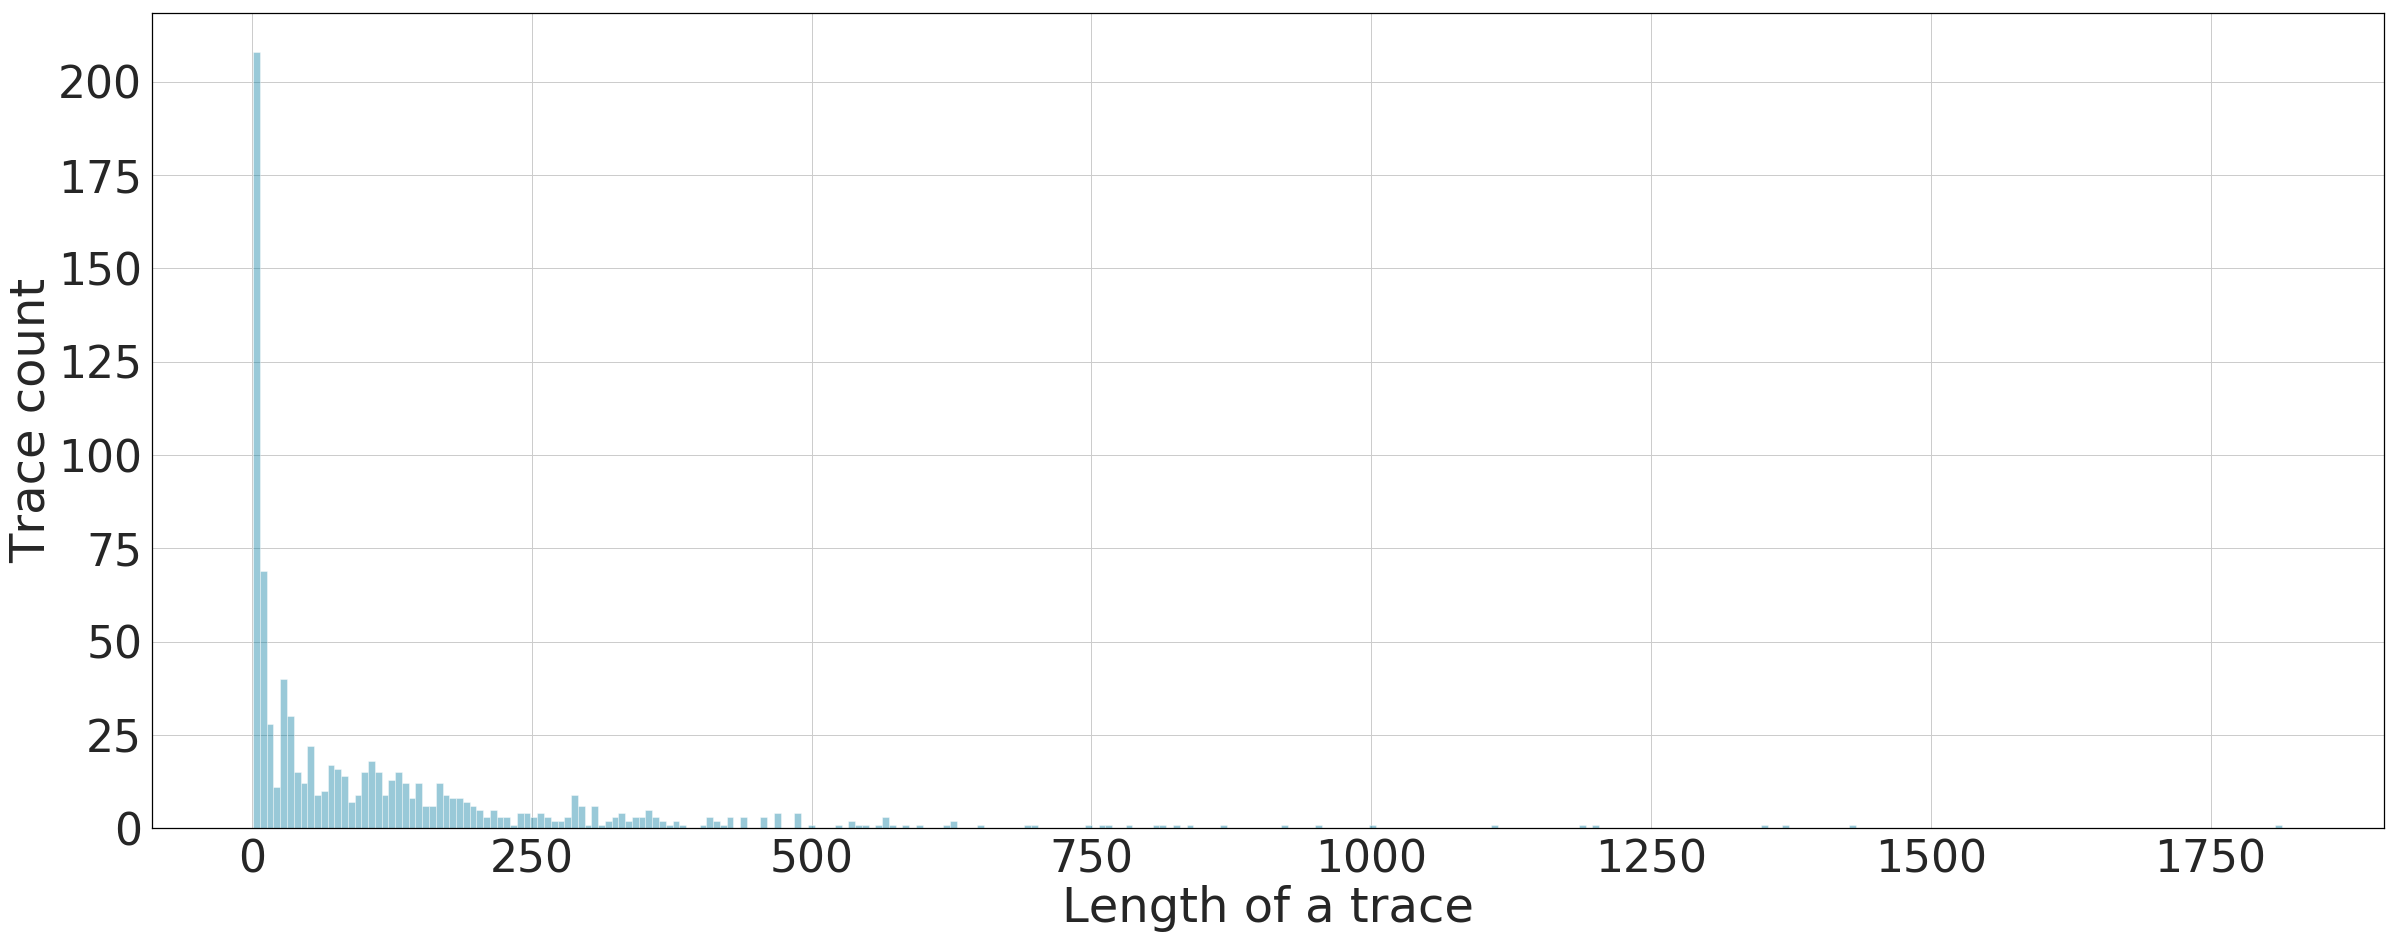
\includegraphics[width=\textwidth]{gfx/frequency-distribution.png}
    \caption{Distribution of trace lengths in the BPIC2011 training set.}
    \label{fig:bpic2011-length-distribution}
\end{figure}

\section{A next-event predictive model training framework}
\label{sec:contrib:training-framework}
\todo[inline]{If Bock and Time}
To bring the four algorithms and four formatting options together, a training framework was implemented which turned out to be easily expandable. Thus we would like to propose it as way to facilitate comparability among prediction approaches.

Data sets

Model builder

Formatter